% inject.tex
\section{Injection of hydrogen into a nitrogen stream}
\label{inject-sec}
%
Figure\,\ref{inject-schematic-fig} shows half of a duct representing
a simple scramjet combustor. 
Nitrogen flows through the duct, from the inflow plane to the outflow plane
(in the $x$-direction), and hydrogen is injected normal to the main flow from
a port in the bottom surface.
The simulated flow domain represents half of the full scramjet duct which is
symmetric about the $y = 0$ plane.

\begin{figure}[htbp]
\begin{center}
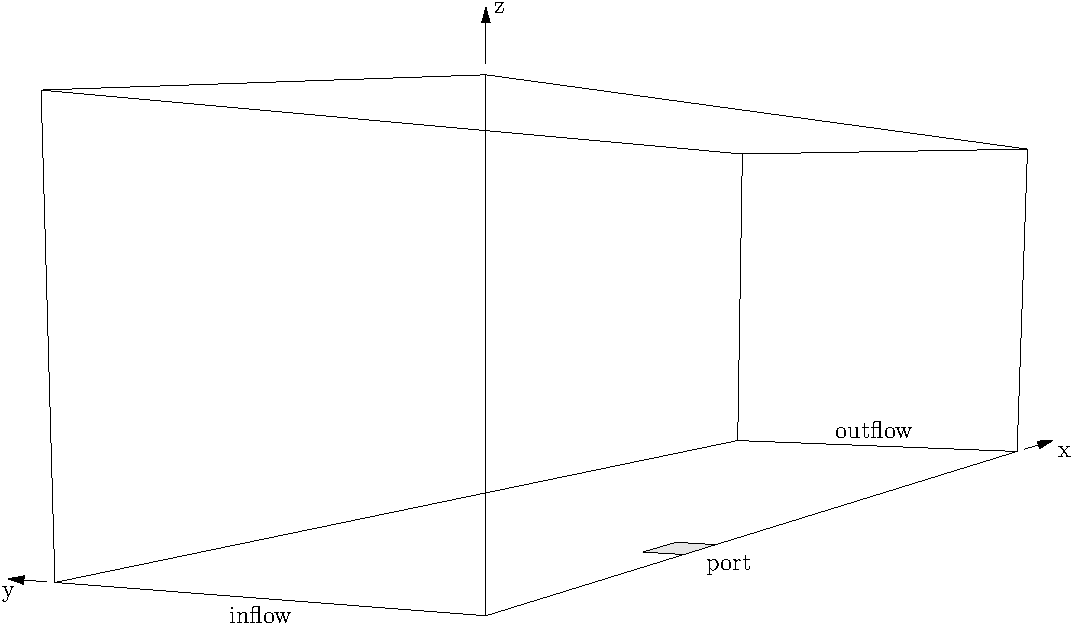
\includegraphics[width=10cm]{../3D/inject-1/inject-schematic.pdf}
\end{center}
\caption{Wireframe representation of the duct with the hydrogen injection port
  shaded on the bottom surface.
  The main stream flow is from the closest (West) boundary to the furtherest
  (East) boundary. }
\label{inject-schematic-fig}
\end{figure}

\medskip
The flow domain consists of 6 blocks filling the whole flow domain as shown in
Figure\,\ref{inject-wireframe-fig}. 
The plan form of the blocks is shown as an ASCII diagram in the middle of
Python input script and has been arranged this way because each block face can
accept only one boundary condition, be it a solid surface or an inflow/outflow
surface.
Thus the inflow of hydrogen is across the whole of the BOTTOM surface of block ``10''.


Figure\,\ref{inject-p-fig} shows the pressure field and the distribution of the hydrogen
jet at a point 3\,ms into the simulation.
With the flow properties selected, the hydrogen jet does not penetrate far
into the main nitrogen stream but the pressure perturbations can can be seen
right across the duct with reflections influencing the downstream part of the hydrogen plume.
This figure was generated with Paraview version 3.8.0 by applying the following filters to the 
full data set:
\begin{itemize}
 \item Cell Data to Point Data
 \item Group Data Sets
 \item Merge Blocks
\end{itemize}
and then the following to the Merge-Blocks data set:
\begin{itemize}
 \item 3 Slice filters, one in each coordinate direction with its cutting plane 
       somewhere near the boundary of the data.  One of these shows massf1 at the exit plane
       and the others show the pressure field on the bottom surface and the symmetry plane through
       the injector.
 \item A contour (value 0.1) of massf1, coloured by p and set at an opacity of 0.6 so that
       the Slice planes show through it.
\end{itemize}


\begin{figure}[htbp]
\begin{center}
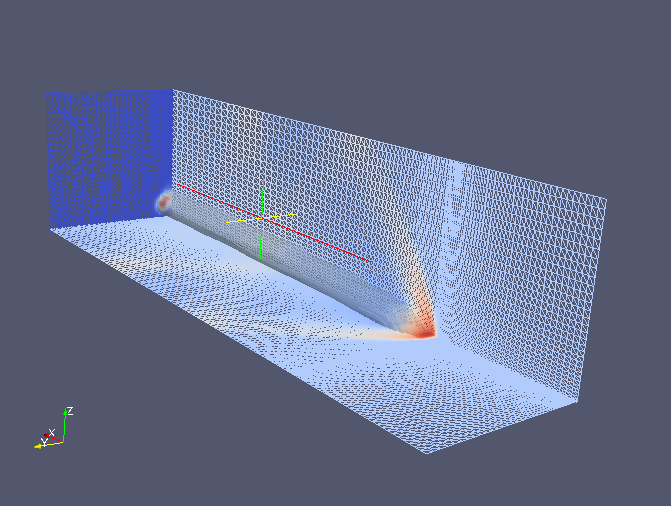
\includegraphics[width=12cm]{../3D/inject-1/inject-p-mesh-on-walls-with-massf1-contour.png}
\end{center}
\caption{Wireframe representation of the surface grid on three surfaces, coloured by pressure on the bottom 
  and symmetry surfaces and coloured by mass fraction on the outflow surface.
  Also plotted is a contour surface for a mass-fraction of hydrogen with a value 0.1, coloured by pressure
  and made partially transparent so that the planar surfaces show through.}
\label{inject-wireframe-fig}
\end{figure}

 
\begin{figure}[htbp]
\begin{center}
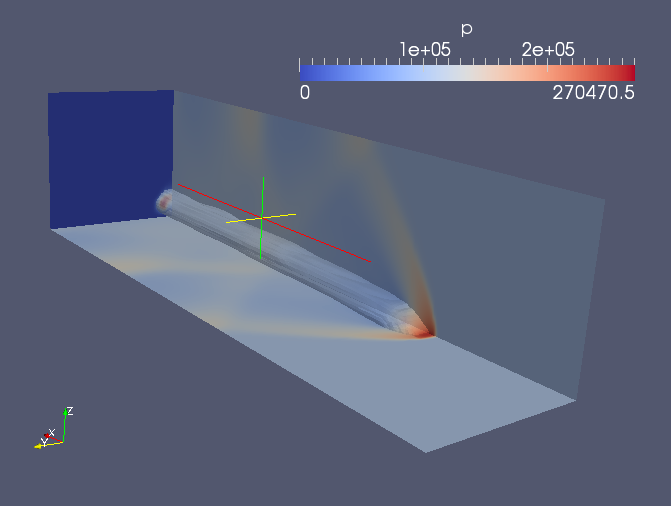
\includegraphics[width=12cm]{../3D/inject-1/inject-p-field-on-walls-with-massf1-contour.png}
\end{center}
\caption{Filled surface representation of pressure and mass-fraction for
  hydrogen at the final time.}
\label{inject-p-fig}
\end{figure}


\newpage

\subsection{Input script (.py)}
\topbar
\lstinputlisting[language={}]{../3D/inject-1/inject.py}
\bottombar


\subsection{Shell script}
\label{inject-sh-files}
\topbar
\lstinputlisting[language={}]{../3D/inject-1/inject_run.sh}
\bottombar


\subsection{Notes}
\begin{itemize}
\item The first part of the input script sets up an ideal-gas mixture model.
  This could have been done separately such that the thermochemistry files
  were already present at the preparation stage.
\item For an ideal-gas model, the run time on 6 cores of \textit{geyser} was 23,987 seconds 
  for 21340 steps.  This is about 1.1 $\mu$s-per-cell-per-update. 
\end{itemize}
